\documentclass[11pt,a4paper]{article}
\usepackage[numbers]{natbib}
\usepackage{graphicx}
\usepackage{subcaption}
\usepackage{amsmath}
\usepackage{amsfonts}
\usepackage{mathtools}
\usepackage{enumitem}
\usepackage{setspace}
\usepackage{adjustbox}
\usepackage{placeins}
\usepackage{booktabs}
\usepackage{tabulary}
\usepackage{hyperref}
\usepackage[capitalise]{cleveref}
\usepackage[a4paper, total={6in, 9in}]{geometry}

\numberwithin{equation}{section}
\creflabelformat{equation}{#2\textup{#1}#3}
\newcommand{\pkg}[1]{{\fontseries{b}\selectfont #1}} 

\bibliographystyle{IEEEtranN}

\title{\textbf{Project step 2: scenario-based stochastic optimisation}}
\author{S. Drake Siard\\
DTU 31792, Spring 2021}
\date{21 Jan 2021}
\begin{document}

\newcommand{\pd}{\ensuremath{p^{D,DA}_d}}
\newcommand{\pdrt}{\ensuremath{p^{D,RT}_{\omega,d}}}
\newcommand{\ud}{\ensuremath{U_d}}
\newcommand{\ushed}{\ensuremath{U_{shed}}}
\newcommand{\pg}{\ensuremath{p^{G,DA}_g}}
\newcommand{\pgrt}{\ensuremath{p^{G,RT}_{\omega,g}}}
\newcommand{\pgspill}{\ensuremath{p^{spill}_{\omega,g}}}
\newcommand{\cg}{\ensuremath{C_g}}
\newcommand{\bnm}{\ensuremath{B_{n,m}}}
\newcommand{\tnm}{\ensuremath{t_{n,m}}}
\newcommand{\fnm}{\ensuremath{f_{n,m}}}
\newcommand{\fnmw}{\ensuremath{f_{\omega,n,m}}}
\newcommand{\FNM}{\ensuremath{F_{n,m}}}
\newcommand{\PG}{\ensuremath{\overline{P}^G_g}}
\newcommand{\PGw}{\ensuremath{\overline{P}^{G,RT}_{\omega,g}}}
\newcommand{\PD}{\ensuremath{\overline{P}^D_d}}
\newcommand{\pw}{\ensuremath{\pi_\omega}}

\maketitle

\section{Problem definition}
\label{sec:problem}
The day-ahead power market-clearing problem with transport constraints from \cite{kazempourLectureMarketClearing2021}, that was solved in step 1 of the project, was extended to include stochastic real-time market clearing as in \cite{kazempourLectureStochasticMarket2021}.

The notation follows a similar convention as before, extended from a single market to the day-ahead and real-time markets.
For a set of generators $\{g\}$ with production costs $\{\cg\}$, demands $\{d\}$ with utility $\{\ud\}$ and common load shedding disutility $\ushed$, buses $\{n\}$, and connections $\{\tnm\}$, denote:
 \begin{itemize}
\item day-ahead generation and consumption as \pg and \pd
\item the set of real-time scenarios as $\Omega$, the individual scenarios as $\omega$, and the corresponding probability $\pw$
\item real-time change in scenario $\omega$ from day-ahead commitment as \pgrt and \pdrt
\item maximum generation for $g$ as $\PG$, maximum demand for $d$ as $\PD$, and maximum flow through connection $\tnm$ as $\FNM$
\item actual wind generation in scenario $\omega$ as $\PGw$
\item the difference in voltage angle between buses $n$ and $m$ as $\theta_n - \theta_m$ (in scenario $\omega$: $\theta_{\omega,n}-\theta_{\omega,m}$), the susceptance of their connection $\tnm$ as $\bnm$, and the (rough) approximation of flow between them as $\fnm = \bnm(\theta_n - \theta_m)$
\item the set of generators and demands in bus $n$ as $\Psi_n$, and the set of buses connected to bus $n$ via transmission lines as $\Omega_n$
\item $\theta_{n_0}$ as the reference voltage angle of some arbitrary bus $n_0$
\end{itemize}

The problem is still the maximisation of social welfare (the sum of the producer and consumer surplus), extended to the real-time market:
\begin{equation}
\max_{\pg,\pd,\theta_n} \left[ \sum_d \ud \pd - \sum_g \cg \pg \right] + 
\sum_\omega \pw \left( \sum_d \ushed \pdrt - \sum_g \cg \pgrt \right)
\end{equation}
In this case $U_{shed}$ is equal to the inferred utility of the inelastic load, \$2000/MW. The objective is optimised subject to both the original day ahead constraints:
\begin{gather}
0 \leq \pd \leq \PD \quad \forall d \label{eq:da_demand} \\
0 \leq \pg \leq \PG \quad \forall g \label{eq:da_supply} \\
-\FNM  \leq \fnm \leq \FNM \quad \forall t_{n,m} \label{eq:da_trans}\\
\theta_{n_0} = 0 \quad \label{eq:prim_ref_theta} \\
\fnm = \bnm(\theta_n - \theta_m) \quad \forall \tnm \label{eq:da_flow} \\
\sum_{d \in \Psi_n} \pd + \sum_{m \in \Omega_n} \fnm - \sum_{g \in \Psi_n} \pg = 0 \quad \forall n \label{eq:da_balance}
\end{gather}
and to the real-time market constraints per scenario:
\begin{gather}
0 \leq \pd + \pdrt \leq \PD \quad \forall \omega, d \label{eq:rt_demand} \\
\pdrt \leq 0 \quad \forall \omega, d \\
0 \leq \pg + \pgrt \leq \PG \quad \forall \omega, g \label{eq:rt_supply} \\
\pgrt = 0 \quad \forall \omega, g \mid g \in \text{inflexible} \\
\pgrt = \PGw - \pg - \pgspill  \quad \forall \omega, g \mid g \in \text{wind} \label{eq:rt_wind} \\
0  \leq \pgspill \leq \PGw \quad \forall \omega, g \mid g \in \text{wind} \\
-\FNM  \leq \fnmw \leq \FNM \quad \forall \omega, t_{n,m} \label{eq:rt_trans}\\
\theta_{\omega, n_0} = 0 \quad \forall \omega \label{eq:prim_ref_theta} \\
\fnmw = \bnm(\theta_{\omega, n} - \theta_{\omega, m}) \quad \forall \omega, \tnm \label{eq:rt_flow} \\
\sum_{d \in \Psi_n} \left( \pd + \pdrt \right) + \sum_{m \in \Omega_n} \fnmw 
- \sum_{g \in \Psi_n} \left( \pg + \pgrt \right) = 0 \quad \forall \omega, n \label{eq:rt_balance}
\end{gather}

Once again, the flows are represented as additional variables with their own bounds (\cref{eq:da_trans,eq:rt_trans}) and explicitly linked to the voltage angles (\cref{eq:da_flow,eq:rt_flow}) for ease of retrieval in the implementation.
Variable wind production is represented as a change in production which will either be used or spilled, with the net change represented by $\pgrt$ (\cref{eq:rt_wind}).
No attempt was made to price flexibility in the objective: it was assumed that flexible real-time generation costs were symmetric and identical to day-ahead costs.
This problem was implemented in MOSEK's Fusion API, as in step 1.

\section{Scenario generation}
\label{sec:scenario}

As before, the day-ahead bid and offer data for 12:00-01:00 on October 7, 2020 from the MISO Market Data site \cite{MISOMarketData} were used as a base, with some additional clean-up (such as excluding generators with the ``Unit Available Flag" unset).
Generators were divided into three categories: flexible, inflexible, and wind; generators with an offer of zero were assumed to be wind, and those with an offer price above the 75th percentile were assumed to be flexible.
Flexible generators were assumed flexible over their entire generation range (from zero to the offered capacity).

For wind generation, MISO historical hourly wind generation data for that hour reported a total of 11937.76 MWh, which was approximately three times the offered capacity attributed to wind generators.
The default scenario was constructed by scaling the bid capacity of each (inferred) wind generator by a common factor so that the total wind capacity matched the historical total wind generation.

To create the scenario sets, reverse forecast error was then applied. 
\cite{hodgeWindPowerForecasting2012} reports the first four moments of forecast error for the ERCOT interconnection in Texas for the year 2010.
By sampling a uniform random variable mapped through the inverse CDF of a distribution\footnote{
See \url{https://www.statsmodels.org/stable/generated/statsmodels.sandbox.distributions.extras.pdf_mvsk.html} for more details.
} matching those moments, a distribution of wind levels that matches the distribution of the empirical forecast error can be derived. 
In order to produce correlated results, one sample per region was combined with one sample per generator to produce the per-generator per-scenario scaler:
\begin{equation}
\epsilon_{g,\omega} = \Phi^{-1}_{\mu,\sigma,s,\kappa} \left( \alpha X_{n,\omega} + (1 - \alpha) X_{g,\omega} \right) \quad \text{where} \quad X_{n,\omega}, X_{g,\omega} \sim U(0,1), \alpha=0.9
\end{equation}
The scaler $\epsilon_g$ was multiplied with the default scenario, and the whole process was repeated 1000 times.
\cref{fig:gen_corr_same} shows the output distribution of two wind generators in the same region, and \cref{fig:gen_corr_diff} shows the joint distribution for generators in different regions.
The univariate distributions are visibly fat-tailed (leptokurtic) and negatively skewed, with a shape directly comparable to \cite{hodgeWindPowerForecasting2012}.

\begin{figure}[htbp]
\centering
\begin{subfigure}{0.45\textwidth}
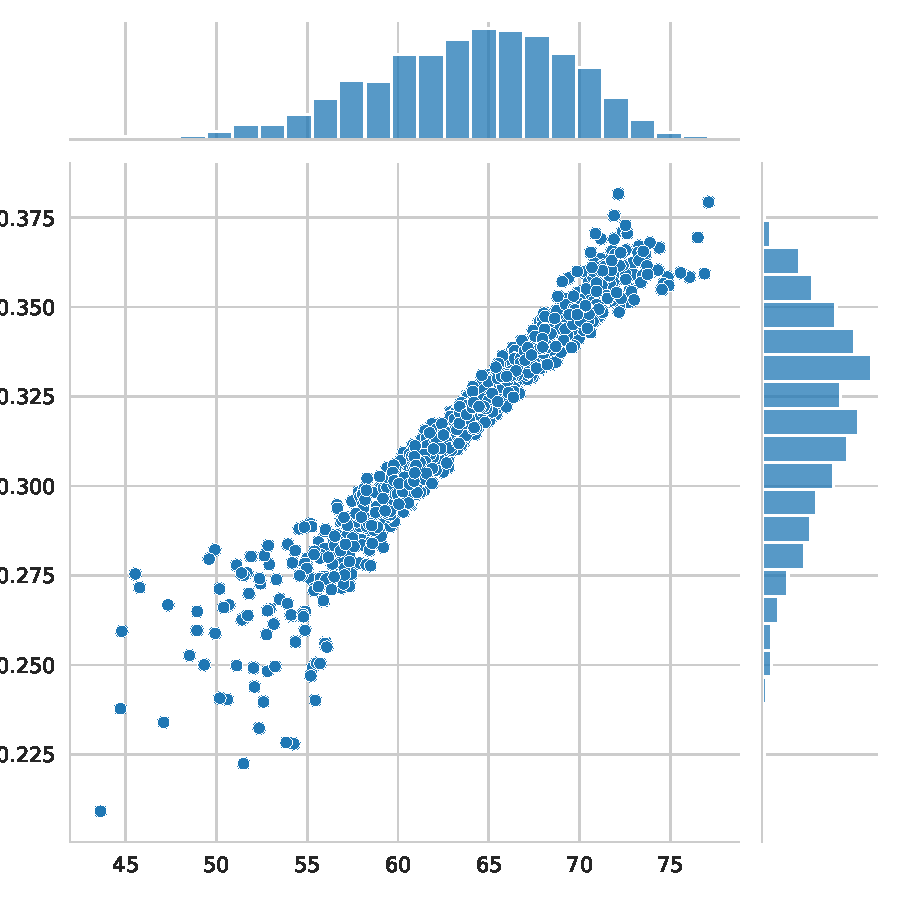
\includegraphics[width=\textwidth]{../output/jointplot_same_region.pdf}
\caption{Same region}
\label{fig:gen_corr_same}
\end{subfigure}%
\begin{subfigure}{0.45\textwidth}
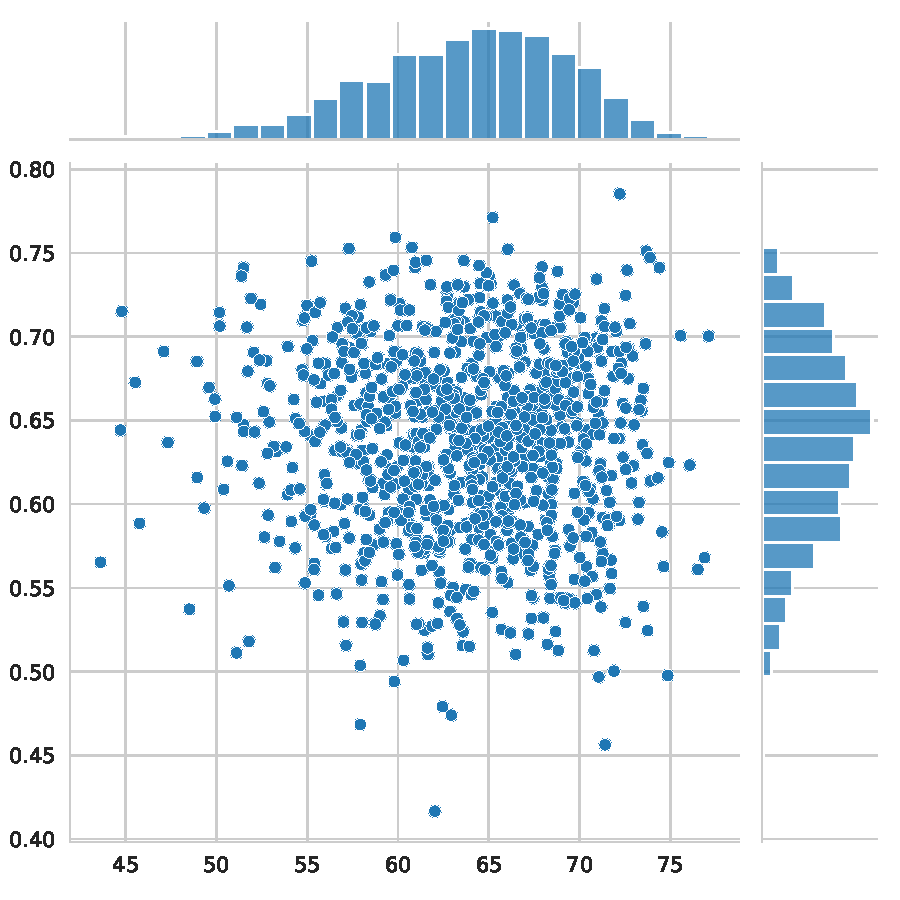
\includegraphics[width=\textwidth]{../output/jointplot_different_region.pdf}
\caption{Different region}
\label{fig:gen_corr_diff}
\end{subfigure}
\caption{Original data correlations}
\end{figure}

\section{Training and testing}

Of the 1000 scenarios, the first 100 were used as a training set, to produce a day-ahead solution, and the remaining 900 as a test and validation set, using the fixed day-ahead solution from the training set\footnote{Implementation in \tt{proj2-stochastic-training.ipynb} and \tt{proj2-stochastic-test.ipynb}}.
The training optimisation, with 346,336 constraints and 349,496 variables (before pre-solving), took 4.8 seconds; the test optimisation, with 3,086,107 constraints and 3,089,267 variables, took 9.1 seconds.
In both cases, the actual optimisation time was dwarfed by the overhead in Python of problem setup, as it was in step 1.

For both the test and training sets, the per-scenario utility was calculated:
\begin{equation}
U_\omega = \left( \sum_d \ud \pd - \sum_g \cg \pg \right) + \left( \sum_d \ushed \pdrt - \sum_g \cg \pgrt \right)
\end{equation}
\cref{fig:obj_dist} shows (normalised) histograms and density plots for the objective values of the test and training sets.
Given that the scenarios are generated with a uniform seed distribution, any random sample of the scenario space is likely to be representative.
In addition, the day-ahead solution from the training set came from a large (100) number of scenarios.
It is therefore no surprise that the per-scenario objective values of the test and training data sets are a close visual match.
More precisely, a (median-centered) Levene test on fails to reject the null hypothesis of equal variance ($p$-value: 0.22), and a two-sample $t$-test fails to reject the null hypothesis of equal means ($p$-value: 0.21).

In summary, given forecast errors in line with the ones used above, the stochastic optimisation produces a something very close to an ideal day-ahead clearing solution.
However, the extreme negative skew of the objective function values suggests that, depending on the system operator's goals, a more robust optimisation technique might be appropriate.

\begin{figure}[htbp]
\centering
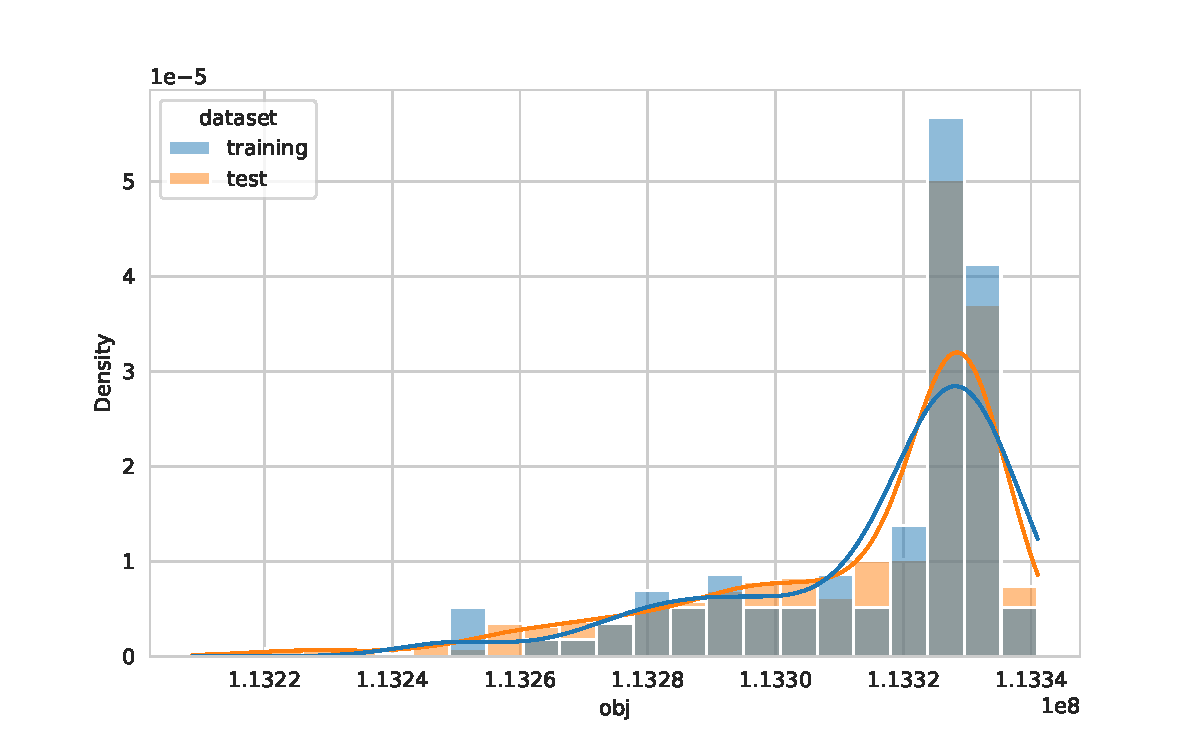
\includegraphics[width=\textwidth]{../output/obj_distribution.pdf}
\caption{Objective function distribution}
\label{fig:obj_dist}
\end{figure}

\renewcommand{\refname}{\section{References}}.
\bibliography{DTU31792}


\end{document}